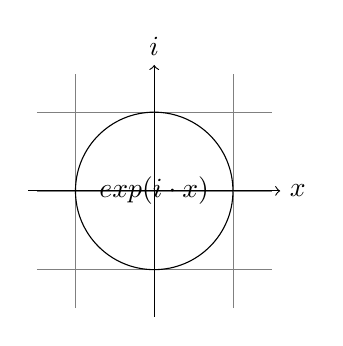
\begin{tikzpicture}[domain=-1.6:1.6]
    \draw[very thin,color=gray] (-1.49,-1.49) grid (1.49,1.49);
    \draw[->] (-1.6,0) -- (1.6,0) node[right] {$x$};
    \draw[->] (0,-1.6) -- (0,1.6) node[above] {$i$};
	\draw (0,0) circle (1cm);
	\node (0.5, 0.5) (expo) {$exp(i \cdot x)$};
\end{tikzpicture}
%Cos-Graph
\begin{tikzpicture}[domain=-4:4]
    \draw[very thin,color=gray] (-4,-1.25) grid (4,1.25);
    \draw[->] (-4,0) -- (4,0) node[right] {$x$};
    \draw[->] (0,-1.25) -- (0,1.25) node[above] {$i$};
	\draw[color=red] plot[id=cos] function{cos(x)} node[below=3.5cm] {\footnotesize $f(x) = cos(x)$};
\end{tikzpicture}

%Sin-Graph
\begin{tikzpicture}[domain=-4:4]
    \draw[very thin,color=gray] (-4,-1.25) grid (4,1.25);
    \draw[->] (-4,0) -- (4,0) node[right] {$x$};
    \draw[->] (0,-1.25) -- (0,1.25) node[above] {$i$};
	\draw[color=red] plot[id=sin] function{sin(x)} node[below=3.5cm] {\footnotesize $f_1(x) =sin(x)$};
\end{tikzpicture}